\section{Preliminaries}
\label{sec:prelim-short}

The main object of study in this paper are $\{0,1\}$-matrices (corresponding to the execution matrix of an algorithm). 
For geometric reasons, we write matrix entries bottom-to-top, i.e.\ the first row is the bottom-most. Thus, $M(i,j)$ is the value in the $i$-th column (left-to-right) and the $j$-th row (bottom-to-top) of $M$. We simultaneously view $M$ as a set of integral points in the plane. For a point $p=(x,y)$, we say that $p \in M$, if $M(x,y) = 1$.
We denote by $p.x$ and $p.y$ the $x$- and $y$-coordinates of point $p$ respectively. 


Given a point set (matrix) $M$, let $p$ and $q$ be points not necessarily
in $M$. Let $\square_{pq}$ be the closed rectangle whose two corners
are $p$ and $q$. Rectangle $\square_{pq}$ is \emph{empty} if
$M \cap \square_{pq} \setminus \{p,q\} = \emptyset$. Rectangle $\square_{pq}$
is \emph{satisfied} if $p,q$ have the same $x$ or $y$ coordinate,
or there is another point $r\in M \cap \square_{pq} \setminus\{p,q\}$.
A point set $M$ is \emph{(arboreally) satisfied} if  
%if for any two points
%$p,q\in M$, 
$\square_{pq}$ is satisfied for any two points $p,q \in M$. %%%The concept of satisfied point sets was introduced in~\cite{DHIKP09}.


\paragraph{Geometric setting for online BST.}

%%\footnote{Should I use the term ``online algorithm'' or ``online BST''?%
%%}


We describe the geometric model for analyzing online BST algorithms (or simply online BST). 
This model is essentially the same as~\cite{DHIKP09}, except for the fact that our model allows cost analysis of  BST algorithms that start accessing an input sequence from arbitrary initial tree.  

For any access sequence $X\in [n]^m$, we also refer to $X$ as an
$n$-by-$m$ matrix, called \emph{access matrix}, where there is a
point $(x,t)\in X$ iff an element $x$ is accessed at time $t$.
We call $(x,t)$ the access point (or input point) at time $t$.
We also refer to the $x$-th column of $X$ as \emph{element} $x$,
and to the $t$-th row of $X$ as \emph{time} $t$. 

For any tree $T$ of depth $d$, let $d(x)$ be the depth of element
$x$ in $T$. We also refer to $T$ as an $n$-by-$d$ matrix, called
\emph{initial tree matrix}, where in each column $x$, there is a
stack of points $(x,1),\dots,(x,d-d(x)+1)\in T$. See \Cref{fig:geo init tree} for an illustration. 
Observe that matrix $T$ is satisfied.

An \emph{online geometric} BST $\cA$ accessing sequence $X$ starting
with initial tree $T$ works as follows. Given a matrix
$\bigl[ \begin{smallmatrix} 
  X\\
  T 
\end{smallmatrix} \bigr]$ 
as input, $\cA$ outputs a satisfied matrix
$\bigl[ \begin{smallmatrix} 
  \cA_{T}(X)\\
  T 
\end{smallmatrix} \bigr]$,
where $\cA_{T}(X)\supseteq X$ is an $n$-by-$m$ matrix called
the \emph{touch matrix} of $\cA$ on $X$ with initial tree $T$.
More precisely, $\aset$ proceeds in an online fashion: At time $t=1,\ldots, n$, the algorithm $\aset$ has access to $T$ as well as to the first $t$ rows of matrix $X$, and it must decide on the $t$-th row of the output $\aset_T(X)$ which cannot be changed afterwards. 
Algorithm $\aset$ is {\em feasible} if  
$\bigl[ \begin{smallmatrix} 
\cA_{T}(X)\\
  T 
\end{smallmatrix} \bigr]$ is satisfied.  

The matrix $\cA_{T}(X)$ can be thought of as the execution log of $\cA$, and points in $\cA_{T}(X)$ are called \emph{touch points}; the \emph{cost} of
$\cA$ is simply $w(\aset_T(X))$, i.e.\ the number of points (ones) in $\cA_{T}(X)$.

An online algorithm with {\em preprocessing} is an online algorithm that is allowed to perform differently at time $t=0$.  
The linear-cost preprocessing used in this paper, as well as in DHIKP~\cite{DHIKP09}, is to put all elements into a \emph{split tree} (see~\cite{DHIKP09} for the details of this data structure). The consequences of this preprocessing are that (i) in the geometric view the initial tree matrix can be removed, i.e.\ an algorithm $\aset$ only gets $X$ as input and outputs $\aset(X)$, and (ii) in the tree-view, an input initial tree $T$ is turned into another tree $T'$ independent of the input $X$, and then keys in $X$ are accessed using the tree-view variant of \greedy. 

DHIKP~\cite{DHIKP09} % 
showed\footnote{with some minor additional argument about initial trees from \Cref{sec:initial-tree}.} that online \emph{geometric} BSTs are essentially equivalent
to online BSTs (in tree-view). In particular, given any online geometric BST 
$\cA$, there is an online BST $\cA'$ where the cost of running
$\cA'$ on any sequence $X$ with any initial tree $T$ is a constant
factor away from $w(\cA_{T}(X))$.
%
Therefore, in this paper, we focus on online geometric BSTs and refer to them from now on simply as online BSTs. 

Unless explicitly stated otherwise, we assume that the access
sequence $X$ is a permutation, i.e.\ each element is accessed only
once, and thus $X$ and $\cA_T(X)$ are $n$-by-$n$ matrices.
This is justified by the following theorem (proof in Appendix~\ref{sec:perm-enough}). 
\begin{theorem}
	\label{thm:perm-all}
	Assume that there is a $c$-competitive geometric BST $\cA^{p}$ for
	all permutations. Then there is a $4c$-competitive geometric
	BST $\cA$ for all access sequences.\footnote{The statement holds unconditionally for offline algorithms, and under a mild assumption if we require $\cA^{p}$ and $\cA$ to be online.}\end{theorem}

\paragraph{\greedy and signed \greedy.}

Next, we describe the algorithms \greedy and signed \greedy~\cite{DHIKP09} (denoted as \sgreedy). 

Consider the execution of an online BST $\cA$ on sequence $X$ with initial
tree $T$ just before time $t$. 
Let $O_{t-1}$ denote the output at time $t-1$ (i.e.\ the initial tree $T$ and the first $t-1$ rows of $\cA_{T}(X)$). 
Let $\tau(b,t-1)=\max\left\{ i\mid(b,i)\in O_{t-1}\right\} $ for any
$b\in[n]$. In words, $\tau(b,t-1)$ is the last time \emph{strictly before} $t$ when $b$ is touched, otherwise it is a non-positive number defined by the initial tree.
Let $(a,t)\in X$ be the access point at time $t$. We define
$\stair_{t}(a)$ as the set of elements $b\in[n]$ for which $\square_{(a,t),(b,\tau(b,t-1))}$
is not satisfied.
\greedy touches element $x \in [n]$ if and only if $x \in \stair_t(a)$.   
See \Cref{fig:geo init tree} for an illustration of stairs.

\begin{figure}[h]
\begin{center}  
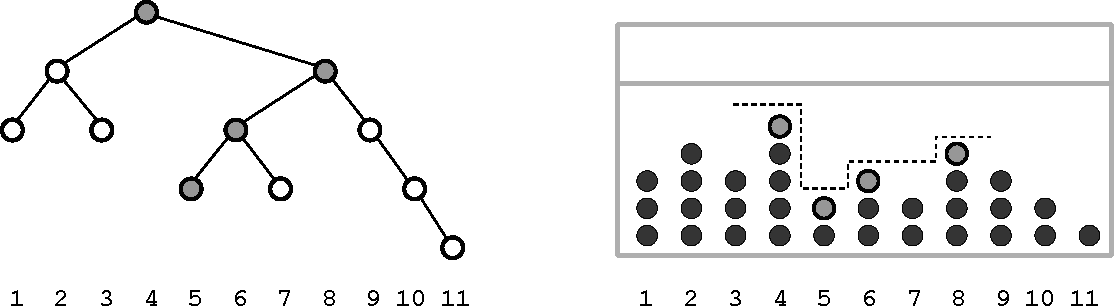
\includegraphics[width=0.65\textwidth]{initial_tree.pdf}
\end{center}
\caption{\label{fig:geo init tree}Tree-view and geometric view of initial tree. Search path and stair (at time 1) of element 5.}
\end{figure}

We define $\stairleft_{t}(a)=\{b\in\stair_{t}(a)\mid b<a\}$
and $\stairright_{t}(a)=\{b\in\stair_{t}(a)\mid b>a\}$. The algorithms \greedyleft
and \greedyright are analogous to \greedy, but they only touch $\stairleft_{t}(a)$, respectively 
$\stairright_{t}(a)$ for every time $t$; \sgreedy simply refers to the union of the \greedyleft and \greedyright outputs, which is not necessarily satisfied. It is known~\cite{DHIKP09, Harmon} that \sgreedy constant-approximates the \emph{independent rectangle bound} which subsumes the two previously known lower bounds on \opt, called Wilber's first and second bounds~\cite{wilber}.
\begin{theorem} [\!\cite{wilber, DHIKP09, Harmon}]
For any BST $\cA$ (online or offline) that runs on sequence $X$ with arbitrary initial tree $T$, $w(\cA_{T}(X))=\Omega(\textsc{SGreedy}(X))$. %
\end{theorem}

A nice property of \greedy and \sgreedy is that an element $x$ can become ``hidden'' in some range in the sense that 
if we do not access in $x$'s hidden range, then $x$ will not be touched. Next, we formally define this concept, and list some cases when elements become hidden during the execution of \greedy and \sgreedy. The concept is illustrated in Figure~\ref{fig:hidden-show}.

\begin{figure}[h]
\begin{center}  
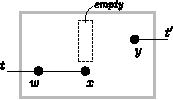
\includegraphics[width=0.35\textwidth]{hidden_ex.pdf}
\end{center}
\caption{\label{fig:hidden-show} After time $t$, element $x$ is hidden in $(w,n]$ for \greedy, and in $(w,x]$ for \greedyright. 
After time $t'$, element $x$ is hidden in $(w,y)$ for \greedy; it is easy to verify that any access outside of $[w,y]$ will never touch $x$.}
\end{figure}


\begin{definition}[Hidden]\label{def:hidden}
	For any algorithm $\cA$, an element $x$ is \emph{hidden in} range $[w,y]$ after $t$ if,
	given that there is no access point $p \in [w,y]\times(t,t']$ for any $t'>t$, then
	 $x$ will not be touched by $\cA$ in time $(t,t']$.
\end{definition}
\begin{lemma} [Proof in Appendix~\ref{sec:wing-hidden}]
\label{prop:hidden}Let $x$ be some element.
\begin{compactenum}[(i)]
\item If there is an element $w<x$ where $\tau(w,t)\ge\tau(x,t)$, then
$x$ is hidden in $(w,n]$ and $(w,x]$ after $t$ for \greedy and \greedyright respectively.
\item If there is an element $y>x$ where $\tau(y,t)\ge\tau(x,t)$, then
$x$ is hidden in $[1,y)$ and $[x,y)$ after $t$ for \greedy and \greedyleft respectively.
\item If there are elements $w,y$ where $w<x<y$, and $\tau(w,t),\tau(y,t)\ge\tau(x,t)$, then
$x$ is hidden in $(w,y)$ after $t$ for \greedy.
\end{compactenum}
\end{lemma}


\paragraph{Forbidden submatrix theory.}

Let $M$ be an $n$-by-$m$ matrix. Given $I \subseteq [n]$ and $J \subseteq [m]$, a \emph{submatrix} $M|_{I,J}$ is obtained by removing columns in $[n] \setminus I$ and rows in $[m] \setminus J$ from $M$.

\begin{definition}
[Forbidden submatrix]Given a matrix $M$ and another matrix
$P$ of size $c\times d$, we say that $M$ \emph{contains}
$P$ if there is a $c\times d$ submatrix $M'$ of $M$ such that
$M'(i,j)=1$ whenever $P(i,j)=1$. We say that $M$ \emph{avoids} (forbids) $P$ if $M$
does not contain $P$. 
\end{definition}

We often call an avoided (forbidden) matrix a ``pattern''. 
For any permutation $\pi = (\pi_1,\dots,\pi_k) \in S_k$, we also refer to $\pi$ as a $k$-by-$k$ matrix where $(\pi_i,i) \in \pi$ for all $1\le i\le k$. % Observe that if an access sequence $S$ avoids a permutation $P$, then the access matrix $S$ is $M_P$-free. 
Permutation matrices have a single one-entry in every row and in every column. Relaxing this condition slightly, we call a matrix that has a single one in every column a \emph{light} matrix. We make use of the following results.
\begin{lemma}
\label{lem:forbidden}
	Let $M$ and $P$ be $n$-by-$n$ and $k$-by-$k$ matrices such that $M$ avoids $P$.  
	\begin{compactenum}[(i)]
		\item (Marcus, Tardos~\cite{marcus_tardos}, Fox~\cite{jfox})\ \  If $P$ is a permutation, the number
		of ones in $M$ is at most $n2^{O(k)}$.
		\item (Nivasch~\cite{nivasch}, Pettie~\cite{pettie_nonlinear})\ \ If $P$ is light, the number of ones in $M$ is at most $n2^{\alpha(n)^{O(k)}}$.
	\end{compactenum}
\end{lemma}	


We define the \emph{tensor product} between matrices as follows: $M \otimes G$ is the matrix obtained by replacing each one-entry of $M$ by a copy of $G$, and replacing each zero-entry of $M$ by an all-zero matrix equal in size with $G$. Suppose that $M$ contains $P$. A \emph{bounding
box} $B$ of $P$ is a minimal submatrix $M|_{I,J}$ such that $P$ is contained in $B$, and $I$ and $J$ are sets of consecutive columns, resp.\ rows. We denote $\min(I)$, $\max(I)$, $\min(J)$, $\max(J)$, as $B.\xmin$, $B.\xmax$, $B.\ymin$, $B.\ymax$, respectively.


